\chapter{Introduction}

\section{Introduction to superfluidity}

The equations of classical fluid dynamics, such as the Navier-Stokes equations, have been known for more than a century. However, the complete understanding of their solutions in a turbulent regime remains one of the most important unsolved problems in classical physics; in particular the statistical and geometric structure of turbulence is still a major topic of current research (see e.g.\ Frisch's review of Kolmogorov theory \cite{frisch1995turbulence}).

With that said, an apparently unrelated topic is quantum mechanics. Bosons are quantum entities that can simultaneusly occupy the same state, unlike fermions because of the Pauli exclusion principle. When a large number of bosons are cooled to temperatures near absolute zero, an intriguing phenomenon occurs: a condensate forms and superfluidity emerges as a macroscopic, coherent quantum state \cite{pitaevskii2016bose}. In such a state, virtually all particles occupy the same quantum state, allowing flow without viscosity and with quantized vortices.

The superfluid can be described by a single macroscopic wave function, which encodes both density and phase (thus velocity) information. Its time evolution is governed by the Gross-Pitaevskii equation (GPE for short), a nonlinear Schrödinger-type equation that accounts for interactions among particles \cite{gross1961structure,pitaevskii1961vortex}. Unlike linear Schrödinger evolution, the nonlinearity in GPE allows phenomena such as vortex cores-regions of near-zero density-around which circulation is quantized.

Despite its quantum nature, the superfluid often exhibits behavior that parallels classical fluid phenomena: quantized vortices move, interact, and can even reconnect, producing structures reminiscent of vortex filaments in classical turbulence \cite{fetter2009rotating}. 

These events though, makes the GPE analitically almost intractable, especially in the presence of multiple vortices or reconnection events. Therefore, it has been widely studied through numerical simulations, (\cite{CZ12,CZ18,CZ21} as just a few examples). 

The aim of this thesis is, therefore, to study in detail an efficient numerical method for solving the GPE in the presence of straight vortices, both from the perspective of numerical analysis and via computational experiments illustrating some examples of straight vortex dynamics. We will employ a time-splitting method combined with finite differences on both uniform and non-uniform grid, which allows for high spatial resolution near the vortex core while keeping the computational cost manageable.

\newpage

\section{The mathematical context}

\subsection{The Gross-Pitaevskii equation}

The governing equation for a weakly interacting Bose-Einstein condendate is, as mentioned before, the \emph{Gross-Pitaevskii equation}

\begin{equation*}
    \ii \hbar \pdv{\psi}{t} = -\frac{\hbar^2}{2m}\lap\psi + V_0\abs{\psi}^2 \psi - E_0 \psi
\end{equation*}

where $\psi = \psi(\rr, t)$ is the complex macroscopic wavefunction for a condensate of $N$ bosons of mass $m$ at position $\rr$ and time $t$. The constant $\hbar$ is the reduced Planck's constant, $V_0$ is the strength of the repulsive interactions between bosons, and $E_0$ is the chemical potential of the system (the energy required to add a boson to the condensate).

The adimensional form of the GPE, whose derivation can be found in \cite{CZ12}, is

\begin{equation}
    \pdv{\psi}{t} = \frac\ii2\lap\psi + \frac\ii2 (1 - \abs{\psi}^2)\psi
    \label{eq:gpe}
\end{equation}

\subsection{Classical analogy via the Madelung transformation}

To give an idea of the analogy with classical fluid mechanics, as previously mentioned, we will give a brief overview of how the GPE can be rearranged to obtain a system of equations that closely resembles the Navier-Stokes equations for an inviscid and incompressible flow.

\medskip

This is achieved through the \emph{Madelung transformation} \cite{madelung1927quantentheorie}, which expresses the complex wavefunction $\psi$ in terms of a real-valued density $\rho$ and a phase $S$ as follows:

\begin{equation}
    \psi(\rr, t) = \rho^{1/2}\exp(\ii S)
    \label{eq:madelung}
\end{equation}

where $\rho = \rho(\rr, t) = \abs{\psi(\rr, t)}^2$ is the density and $S = S(\rr, t)$ is the phase of $\psi$. The vector field $\uu = \nb S$ can be interpreted as the superfluid velocity field.

\medskip

Substituting \eqref{eq:madelung} into \eqref{eq:gpe} and separating real and imaginary parts, after some straightforward algebra \cite{CZ12}, we obtain the following system of equations, written in tensorial notation

\begin{align*}
    &\pdv{\rho}{t} + \pdv{(\rho u_j)}{x_j} = 0 \\
    &\rho \left(\pdv{u_i}{t} + u_j \pdv{u_i}{x_j}\right) = -\pdv{p}{x_i} + \pdv{\tau_{ij}}{x_j}, \quad i = 1,2,3
\end{align*}

where 

\[
    p = \frac{\rho^2}{4} \quad \text{and} \quad \tau_{ij} = \frac14 \rho \frac{\partial^2\,\log \rho}{\partial\,x_i x_j}
\]

are the pressure and the quantum stress tensor, respectively.

We can clearly recognize the mass continuity equation in the first equation, being formally identical to its classical counterpart. Differences begin to emerge in the second equation, which essentially expresses the conservation of momentum.

The quantum fluid is inherently \emph{inviscid}. Unlike the viscous stress tensor $d_{ij}$ \cite{noteZ} present in the Navier-Stokes equations, which is proportional to the velocity gradient and dissipates kinetic energy through friction, while the \emph{quantum stress tensor $\tau_{ij}$} introduces no dissipation. Instead, this term redistribute the energy within the system \cite{Tanogami2021}.

These deep formal similarities suggest that the study of quantum vortex dynamics, in particular \emph{non-dissipative vortex reconnection} events, could provide valuable insights into understanding the complex structure of turbulence in the classical case.

\section{Approximation of steady-state vortex}

In what follows, we will focus on the two-dimensional case, which is sufficient to describe straight vortices in three dimensions. Here we will seek an expression for the density profile in the case of a single steady-state vortex, centered at the origin. Let us start by imposing that and the time independency. In a 2-dimensional domain, with these constraints, the wavefunction has the form

\[
    \psi(x,y)=f(r)\exp\left(\ii\,\theta(x,y)\right)
\]

where $r = \sqrt{x^2 + y^2}$ and $f(r) = \sqrt{\rho(r)}$.

Now, we need to determine the function $f(r)$. By imposing the time independency condition, and substituting the above expression into the GPE \eqref{eq:gpe}, we obtain the following boundary value problem:

\begin{equation}
    f'' + \frac{f'}{r} + f\left(1 - f^2 - \frac{1}{r^2}\right) = 0
    \label{eq:density}
\end{equation}

with boundary conditions $f(0)=0$ and $f(\infty)=1$. There are several approaches: one could solve the boundary-value problem directly on a truncated domain and interpolate the solution. In many applications, however, it is convenient to approximate $f(r)$ using a Padé approximant \cite{Berloff20041617}, in order to be able to evaluate the function everywhere. In what follows we will use a 4-th order Padé approximant, which coefficients can be found in \cite{CZ18}.

\begin{figure}[H]
    \centering
    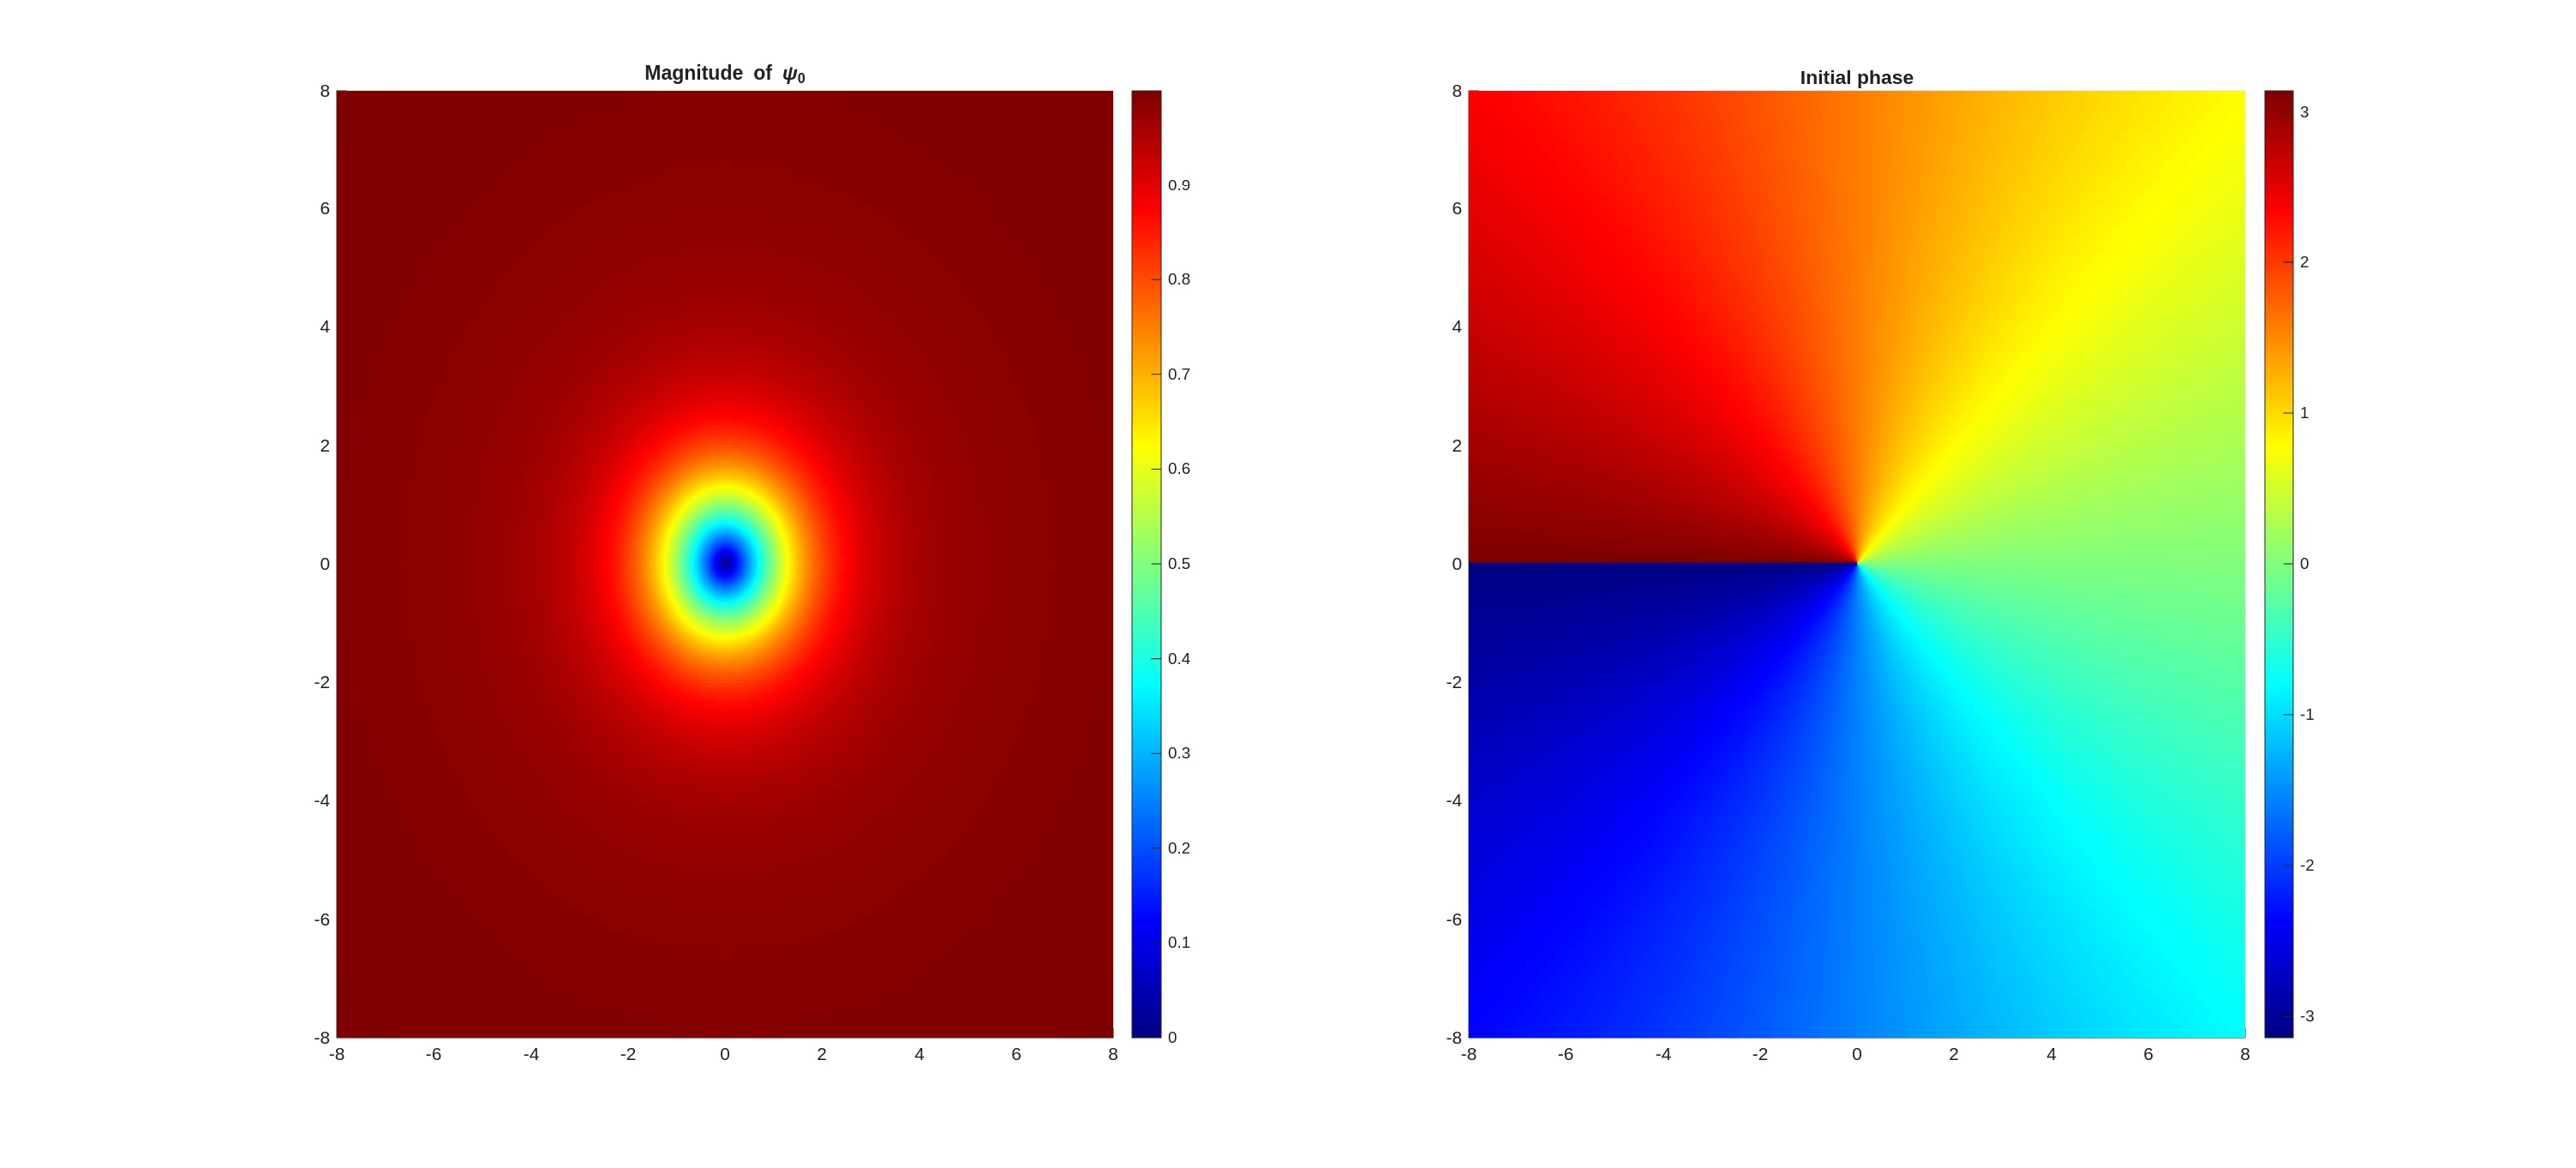
\includegraphics[width=\textwidth]{img/initial_cond.pdf}
    \caption{Magnitude $\abs{\psi_0} = \sqrt{\rho}$ (left), initial phase in radiants (right)}
\end{figure}


